\documentclass[]{scrartcl}
\title{Vorlesung Analysis II}
\usepackage{amsmath,amssymb,amsfonts}
\usepackage{stmaryrd}
\usepackage{mathtools}
\usepackage{latexsym}
\usepackage{graphicx}
\usepackage{tikz}
\usepackage{xcolor}
\usepackage{soul}
\usepackage{hyperref}
\usepackage{tipa}
\usepackage[normalem]{ulem}
\usepackage[dvipsnames]{xcolor}
\hypersetup{
	colorlinks=true,
	linkcolor=blue,
	filecolor=magenta,      
	urlcolor=cyan,
	pdftitle={Overleaf Example},
	pdfpagemode=FullScreen,
}
\newcommand{\redcircle}[1]{%
	\tikz[baseline=(char.base)]{
		\node[shape=circle, draw=red, text=red, thick, inner sep=1pt] (char) 
		{\textbf{#1}};
	}%
}
\setul{1pt}{3pt} % Linienhöhe und Abstand zum Text (optional anpassbar)

\setlength{\topmargin}{-.5in} \setlength{\textheight}{9.25in}
\setlength{\oddsidemargin}{0in} \setlength{\textwidth}{6.8in}
\setlength{\parindent}{0pt}

\begin{document}
	\textbf{\underline{Teil 2: Topologische Grundbegriffe in metrischen Räumen}}\\
	\\
	\textbf{\underline{an12:Konvergenz und Kompaktheit}}\\
	\\
	\textbf{\underline{\underline{Stichworte:} Vollständigkeit, allg. Banach-Fixpunktsatz, Kompaktheit, Heine-Borel}}\\
	\\
	\underline{Literatur:} \setulcolor{blue} \ul{[Forster], Kapitel 3}\\
	\\
	\textbf{12.1. \underline{Einleitung:}} $\mathbb{R}^n$ ist als metrischer Raum vollständig. Wir zeigen, dass abgeschlossene Teilmengen eines vollständigen metrischen Raums wieder Vollständig sind, was einen neuen Blick auf den Banachschen Fixpunktsatz wirft.
	Weiter werden wir zum Kompaktheitsbegriff geführt, und wir zeigen den Satz von Heine-Borel, welcher besagt, dass die (überdeckungs-)kompakten Teilmengen im metrischen Raum $\mathbb{R}^n$ genau die sin,  die beschränkt und abgeschlossen sind.\\
	\\
	\textbf{12.2 \underline{Motivation:}} Sei $\o \neq M \subseteq (R,\delta)$, dann ist \setulcolor{green} \ul{$(M,\delta_{\neg MxM})$ auch metrischer Raum.}\\
	Für $a \in M$ ist dann eine Kugel in M um a:\\
	\setulcolor{yellow} \ul{$B_{a,n}^\epsilon$}:=$\{x\in\mathbb{R};\delta(x,a)<\epsilon\}\cap M = B_{a,R}^\epsilon\cap M.$\\
	\begin{figure}[h]
		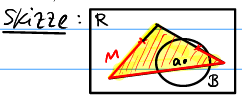
\includegraphics[width=7 cm,height=3cm]{bsp kap 12.2}
	\end{figure}\\
	\underline{Beobachtung:} $B_{a,n}^\epsilon$ offen in M, i.a. aber nicht in R.\\
	\\
	\textbf{12.3 \underline{Bezeichnung:}} in M \setulcolor{red} \ul{relativ offen} :$\Leftrightarrow$ offen in M\\
	in M \ul{relativ abgeschlossen}:$\Leftrightarrow$ abg. in M\\
	\\
	\textbf{12.4} Es gibt: \\
	$M\supseteq U$ \setulcolor{green} \ul{odden in M} $\Leftrightarrow$ \ul{$O \in \mathcal{O}(R):U=O\cap M$},\\
	$M\supseteq U$ \ul{abg. in M} $\Leftrightarrow$ \ul{$\exists A \in \mathcal{A} (R):A\cap M$}.\\
	\\
	\textbf{12.5. \underline{Bem.:}} Sei $a\in M \subseteq R.$\\
	(1) \ul{$a\in \dot{M}$} $\Leftrightarrow \forall k \in \mathbb{N}$ \ul{$\exists x_k \in M \backslash\{a\}:x_k\rightarrow a$},\\
	(2) \ul{$a \in \overline{M}$} $\Leftrightarrow \forall k \in \mathbb{N}$ \ul{$\exists x_k \in M: x_k \rightarrow a$}.\\
	\underline{Bew.:} Zu (1): "$\Rightarrow$: $a \in \dot{M} \Rightarrow \exists x_k \in (U_a^{\frac{1}{k}}\backslash\{a\})\cap M \Rightarrow x_k\rightarrow a.$\\
	"$\Leftrightarrow$" vgl. Def. HP in \setulcolor{blue}\ul{11.14}: In jeder Umgebung von $x_k$ lieden $\infty$ viele Folgenglieder $\Rightarrow$ a ist HP.\\
	Zu (2): $\overline{M} = M\cup \dot{M}$ aus \ul{(1)}.\\
	\\
	\textbf{12.6. \underline{Satz:}}(R.S) \setulcolor{green}\ul{vollständig, $M\subseteq R$}.\\
	\underline{Beh.:} \ul{M vollständig $\Leftrightarrow$ M Abgeschlossen}.\\
	\underline{Bew.:}"$\Rightarrow$": Zeige $M=\overline{M}$ oder: $a\in\overline{M} \xRightarrow{12.3(2)} \exists(x_k)\subseteq M, x_k \rightarrow a \Rightarrow (x_k)$ ist CF\\
	$\Rightarrow$a = $lim x_k \in M,$ da M vollständig nach Vor.\\
	"$\Leftarrow$":$(x_k)$ CF in M $\Rightarrow (x_k)$ CF in $R\Rightarrow \exists a \in R: x_k \rightarrow a \Rightarrow a\in \overline{M}=M.$\\
	\strut\hfill$\square$\\
	Wir erhalten weiter die allgemeine Version der Banachschen Fixpunktsatzes in \underline{vollständigen} metrischen Räumen wie folgt.\\
	\\
	\textbf{12.7. \setulcolor{red}\ul{Banachscher Fixpunktsatz(allg. Version):}}\\
	\underline{Vor.:} $(R,\delta)$ \setulcolor{green}\ul{vollständiger metrischer} Raum, f: \ul{$R\rightarrow R$ Kontraktion} mit Kontraktionsfaktor $p\in[0,1[.$\\
	\underline{Beh.:} \\
	a) \ul{$\exists!$ Fixpunkt a von f}.\\
	b) Setze \ul{$x_0 \in R$} beliebig und \ul{$x_{k+1} := f(x_k)$} für alle k $\geq$0.\\
	Dann: \ul{$\delta(x_k,a) \leq \frac{p^k}{1-p}\delta(x_1,x_0)$}, d.h. insb. \ul{$\lim_{k\rightarrow\infty}x_k=a$}.\\
	\\
	\underline{Bew.:} Wie in \setulcolor{blue} \ul{8.6} zeigt mann, dass ($x_k$) eine CF ist.\\
	Da R vollständig, ex. $a=\lim_{k\rightarrow\infty}x_k \in R.$ wie dort zeigt man f(a)=a.\\
	\strut\hfill$\square$\\
	\textbf{12.8 \underline{Bem.:}} Da der frühere Fixpunktsatz für Kontraktionen auf $U \subseteq \mathbb{R}^n$ formuliert ist, wo U abg. \sout{und beschr. ist(also Kompakt nach kap 12.11)} und somit vollständig nach \ul{12.6}, und \ul{\redcircle{Ü} Bl. 2A2.2}\setulcolor{green}(\ul{$\mathbb{R}^n$ ist vollständig}), folgt die alte version \setulcolor{blue} \ul{8.6} auch aus \ul{12.7}.\\
	\\
	Für bestimmte Anwendungen(z.b Existenz von Extrema auf bestimmten Teilmengen des $\mathbb{R}^n$) reicht die Abgeschlossenheit oft nicht aus, wir benötigen dafür einen stärkeren Begriff wie folgt.\\
	\\
	
	
	
	
	
	
\end{document} 
